\chapter{{\cpunet} Results}\label{chap:cpu_net_result}

\section{Introduction}
In order to have accurate simulations, the ATN needs to reproduce the correct ensemble distribution of the parameters used in PSD. Since {\onbb} events are single-site events, LEGEND seeks to distinguish between single-site and multi-site events using PSD techniques. We trained {\cpunet} on 110,000 FEP waveforms and then used 1,200 SEP events and 3,000 DEP events for validation. In this chapter, we present the results of ATN's ability to reproduce detector waveforms using some critical parameters used in PSD. 

\section{Training progression}
The progression of training losses is shown in figure \ref{fig:training_loss}. The cycle-consistent and identity losses converge rapidly towards zero. The adversarial training is evident in the losses for the discriminators and generators. During training, the discriminator initially wins, and its loss decreases while the generator's loss increases. As training continues, the generator catches up, and the networks approach an equilibrium in which each attempts to out-compete the other. Thus, the loss functions fluctuate as they continuously adapt and improve.

\begin{figure}%[htb!]
    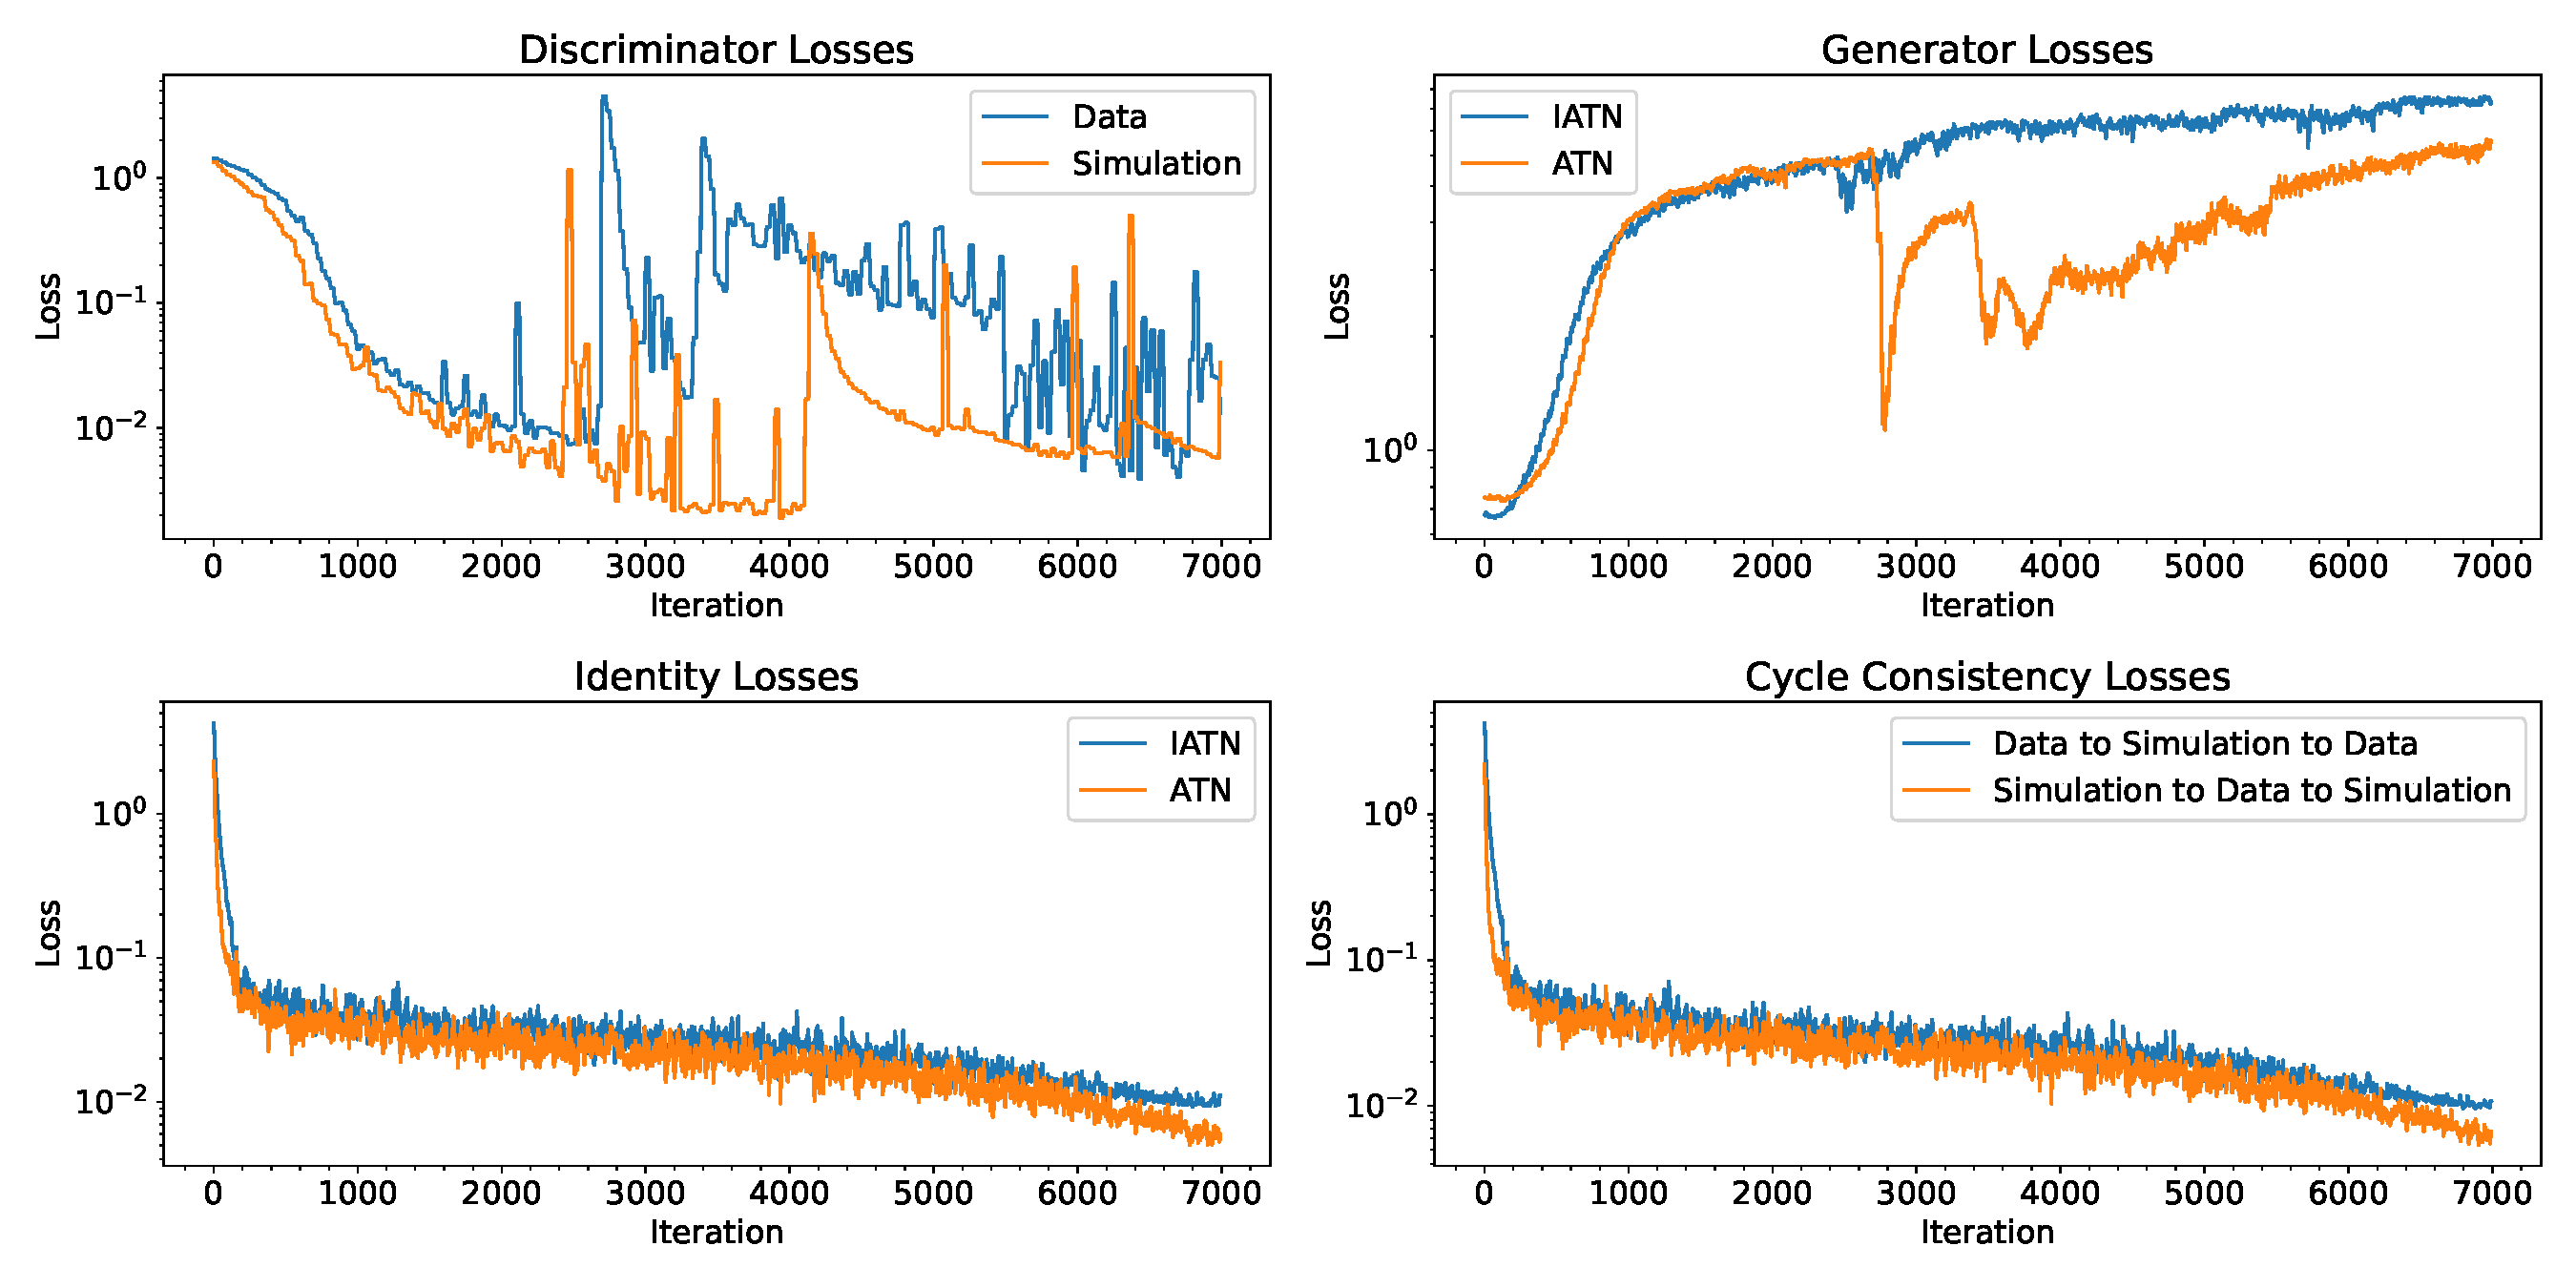
\includegraphics[width=\linewidth,trim={0.5cm 0pc 0.5cm 0pc},clip]{ch8/figs/loss_funcs.pdf}
    \caption{Training losses for {\cpunet}. Losses have been smoothed using a moving average of 10 samples for clarity. The identity and cycle losses rapidly converged to zero while the generator and discriminator losses fluctuate.} 
   \label{fig:training_loss}
\end{figure}


\section{Waveform Translation}
The translation of the simulated waveform is shown in figure \ref{fig:current_amp}. The ATN translates the simulated waveform to the ATN output by smoothing the sharp turning edge in the orange region. This is a consequence of the non-zero integration time in detector waveforms, which is set to $0$ in {\siggen}. The RC discharge effect of the electronics readout system is also set to 0 in {\siggen}, leading to a tail slope of 0 in the simulated waveforms. The ATN learns to translate the flat tail in the cyan region into exponential decay.

\begin{figure}[htb!]
    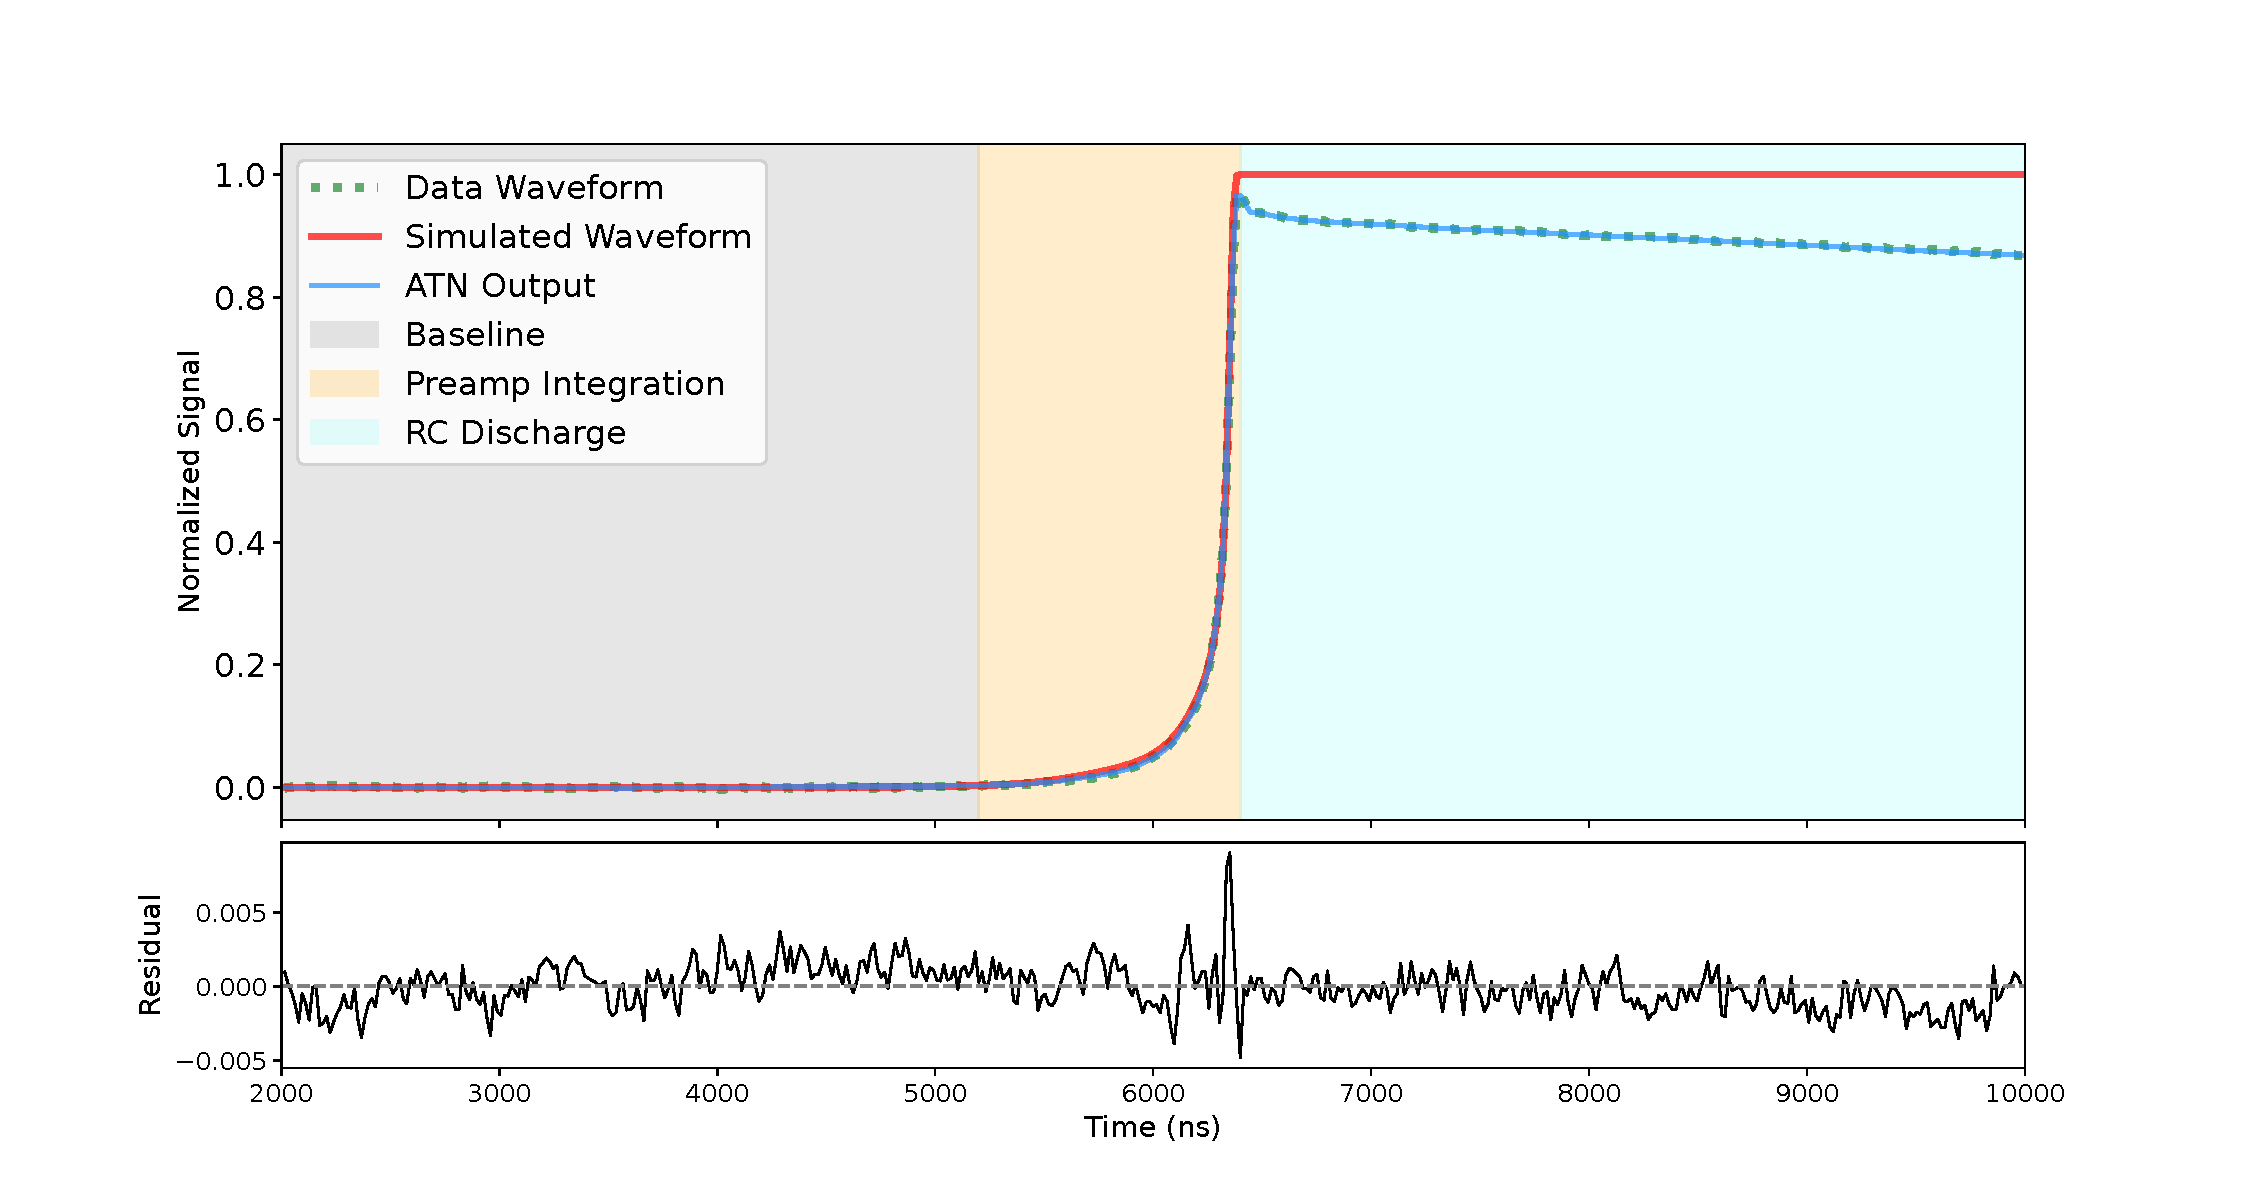
\includegraphics[width=\linewidth,trim={2.0cm 0pc 3.0cm 0pc},clip]{ch8/figs/wf_comp_sim_atn_data.pdf}
    \caption{An example ATN output (blue) generated by the input simulated waveform (red). A detector waveform (dotted green), manually selected from data to resemble the ATN output, is included for reference. The orange region depicts the area where the preamplifier integration effect is most visible. The blue region shows the impact of the RC circuit discharge effect. Grey region shows the baseline region with electronics noise. A residual panel comparing the ATN output to the reference waveform is included below. A 0 residue is not expected, as the reference waveform is not a one-to-one match with the simulated waveform.} 

   \label{fig:sample_result}
\end{figure}

Figures \ref{fig:cycle_bab} and \ref{fig:cycle_aba} show the SEP waveforms as they progress through the cycle in {\cpunet}. The network effectively translates the waveforms in forward and reverse translations. In the {\siggen} simulations, the RC discharge effect is not modeled, resulting in a flat tail slope of zero. ATN learns to transform this flat tail into an exponentially decaying one while including more subtle effects like overshoot and a faster decay early in the tail, matching the observed behavior in real detector data, and IATN learns to transform it back to a zero slope, matching the simulations.

\begin{figure}%[htb!]
    \centering
    %trim={0pc 0pc 0pc 3pc},clip
    \includegraphics[width=0.99\linewidth]{ch8/figs/SEP_result_comp_1x3_cycle_BAB.pdf}
    \caption{Cycle consistency in waveform translation in forward direction. Starting with 10 simulated waveforms, the ATN first translates them into detector-like waveforms, and then IATN translates them back to the simulation like waveforms.}
    \label{fig:cycle_bab}
\end{figure}

\begin{figure}%[htb!]
    \centering
    %trim={0pc 0pc 0pc 3pc},clip
    \includegraphics[width=0.99\linewidth]{ch8/figs/SEP_result_comp_1x3_cycle_ABA.pdf}
    \caption{Cycle consistency in waveform translation in backward direction. Beginning with 10 detector waveforms, the IATN translates them into simulated-like waveforms, and then ATN translates back to detector-like waveforms.}
    \label{fig:cycle_aba}
\end{figure}

\section{Validation of Key Waveform Parameters}
 The accuracy of translations can be assessed at a distribution level by plotting the histogram of key reconstruction parameters. We use the Intersection over Union (IoU) metric, also known as the Jaccard index, to measure the overlap between distributions $A$ and $B$ \cite{murphy1996finley, jaccard_index}. We first calculate the histogram of the distribution being compared using the same binning. The \textit{intersection} is $\sum_{i} \min(\text{bin}_i^A, \text{bin}_i^B)$, the \textit{union} is $\sum_{i} \max(\text{bin}_i^A, \text{bin}_i^B)$, and
 
\begin{equation}
  \text{IoU} \;=\; \frac{\sum_{i} \min(\text{bin}_i^A, \text{bin}_i^B)}{\sum_{i} \max(\text{bin}_i^A, \text{bin}_i^B)}.    
\end{equation}
We express the result in percentages. An IoU of $100\%$ indicates perfect agreement and $0\%$ indicates no agreement between the histograms.
 
\subsection{Drift Time Distribution}
The electric field of the HPGe detector allows events at different locations to have unique waveform shapes, allowing reconstruction of the event topology. As shown in figure \ref{ch7_fig_eng_dep_sim}, each location has a different drift time, making it a crucial parameter for waveform analysis. Overall, data waveforms have a longer drift time than simulations because of the integration of the preamplifier. To calculate the drift time, we define two time points shown in figure \ref{fig_ch8_time_calc}. tp$1$ is defined as the time the waveform reached $1\%$ of its maximum value, and tp$100$ represents the time the waveform reached its maximum value. The time points are found by first finding the maximum time point and then searching backward to find the point when the waveform first crosses that amplitude. The drift time $T_{Drift}$ of the waveform is the time between the two points. 

\begin{figure}%[!htb]
    \centering
    %trim={0pc 0pc 0pc 3pc},clip
    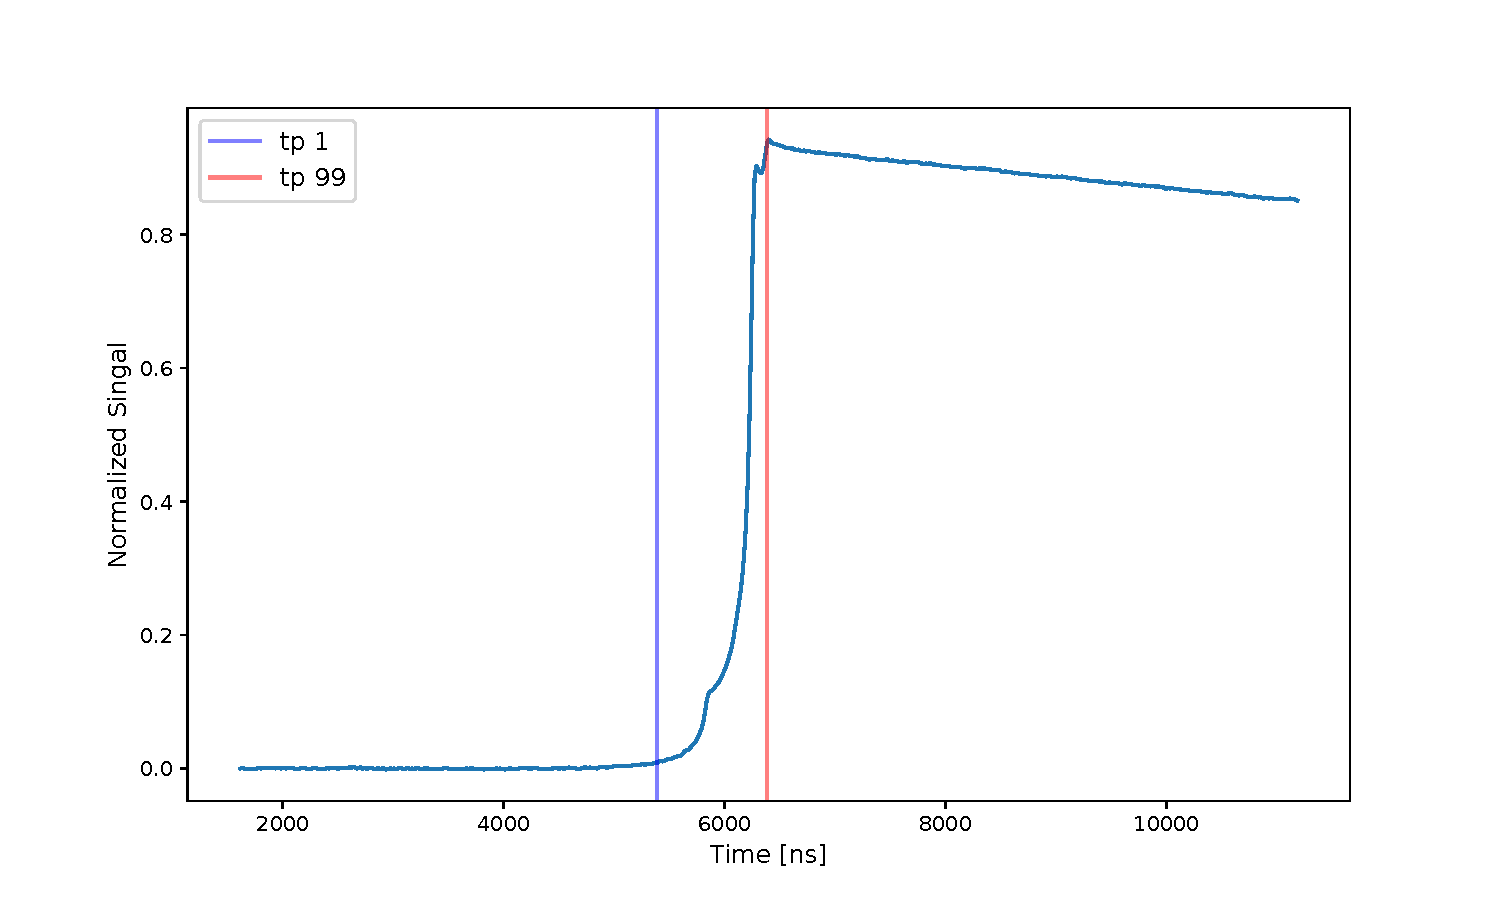
\includegraphics[width=0.9\linewidth]{ch8/figs/time_calc.pdf}
    \caption{Calculating the time points of the waveform.}
    \label{fig_ch8_time_calc}
\end{figure}

Figures \ref{fig:drift_times_sep} and \ref{fig:drift_times_dep} illustrate the distribution of $T_{Drift}$ in the SEP and DEP validation datasets. ATN nets learn to slow the drift time of the simulated waveforms to match the distribution of the data.  The SEP $T_{Drift}$ IoU increases to $62.4\%$ from $39.5\%$. The DEP IoU increases to $22.5\%$ from $5.4\%$.
 
\begin{figure}%[!htb]
%[trim={left bottom right top},clip]
\centering
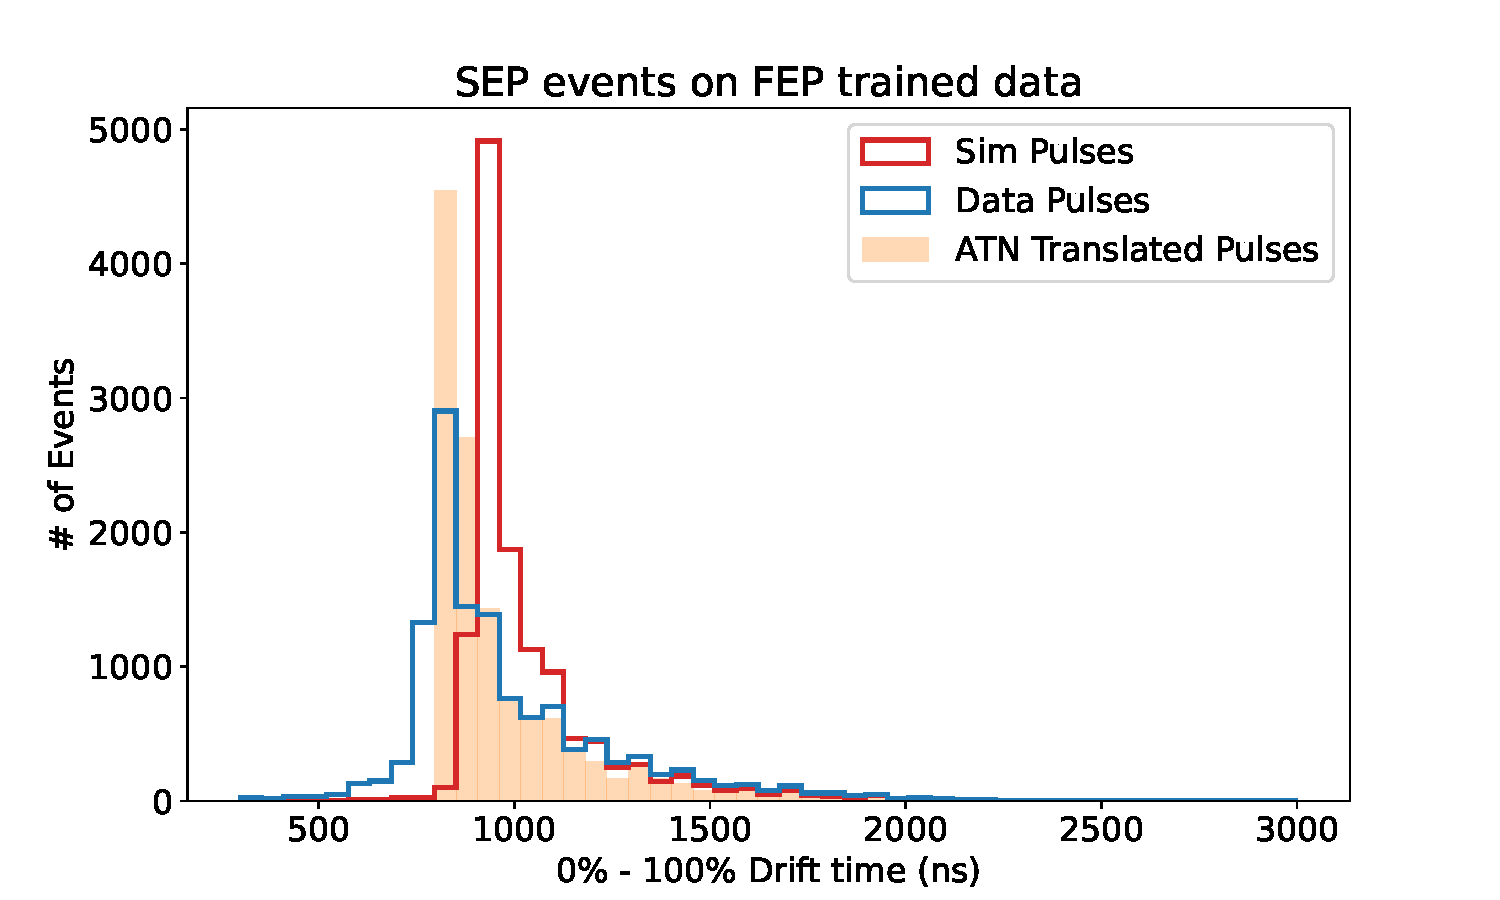
\includegraphics[width=0.9\linewidth,trim={0pc 0pc 0pc 0pc},clip]{ch8/figs/sep_drift_time.pdf}
\caption{The distribution of the 1\%–100\% drift time on SEP dataset.}
\label{fig:drift_times_sep}
\end{figure}

\begin{figure}%[!htb]
%[trim={left bottom right top},clip]
\centering
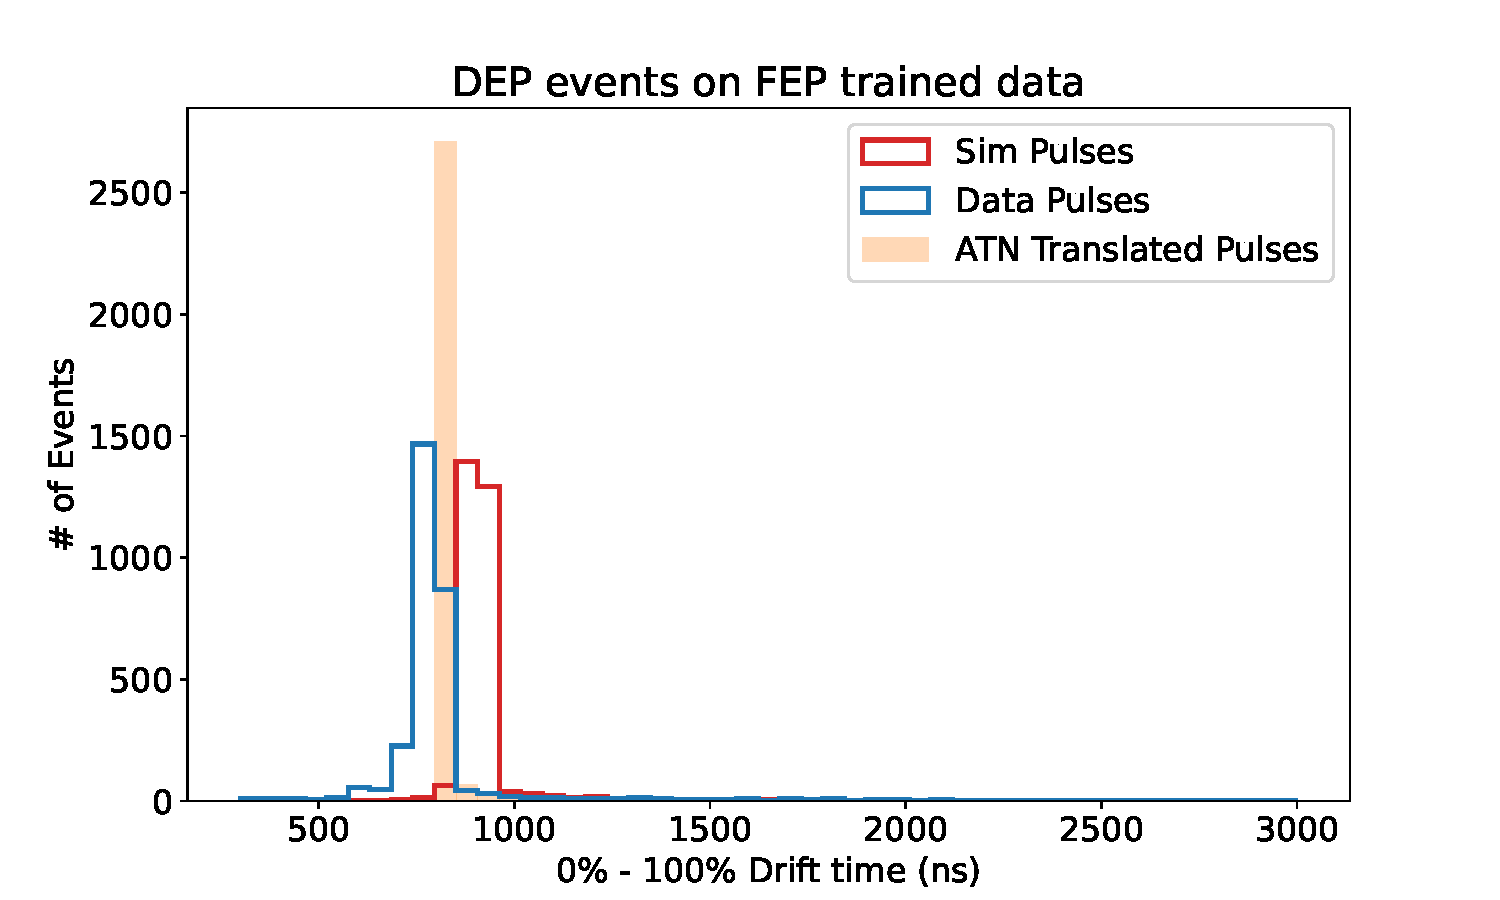
\includegraphics[width=0.9\linewidth,trim={0pc 0pc 0pc 0pc},clip]{ch8/figs/dep_drift_time.pdf}
\caption{The distribution of the 1\%–100\% drift time on DEP dataset.}
\label{fig:drift_times_dep}
\end{figure}

\subsection{Current Amplitude}
For a given event energy, single-site events produce a localized energy deposition, resulting in a sharper and faster increase in $I_{max}$. In contrast, multi-site events, characterized by energy deposition at multiple locations within the detector, yielding the same current spread over multiple peaks, decreasing the magnitude of the maximum current value. This distinction makes $I_{max}$ highly effective in differentiating single-site from multi-site events, thereby establishing it as a crucial parameter in waveform shape simulations \cite{mjd_psd}.

The maximum current amplitude $I_{max}$ is determined by differentiating the waveform and identifying the maximum value of its derivative. Fig.\ref{fig_ch8_curr_amp_calc} shows the steps taken to calculate the current amplitude. The waveform example used here is from an event that deposited energy in two locations in the detector. The current amplitude thus has two peaks. Then the maximum current would be lower than one for a single-site event, which would only have a single peak and thus higher $I_{max}$. This is why current amplitude is highly accurate in distinguishing single- and multi-site events.


\begin{figure}%[!htb]
    \centering
    %[trim={left bottom right top},clip]
    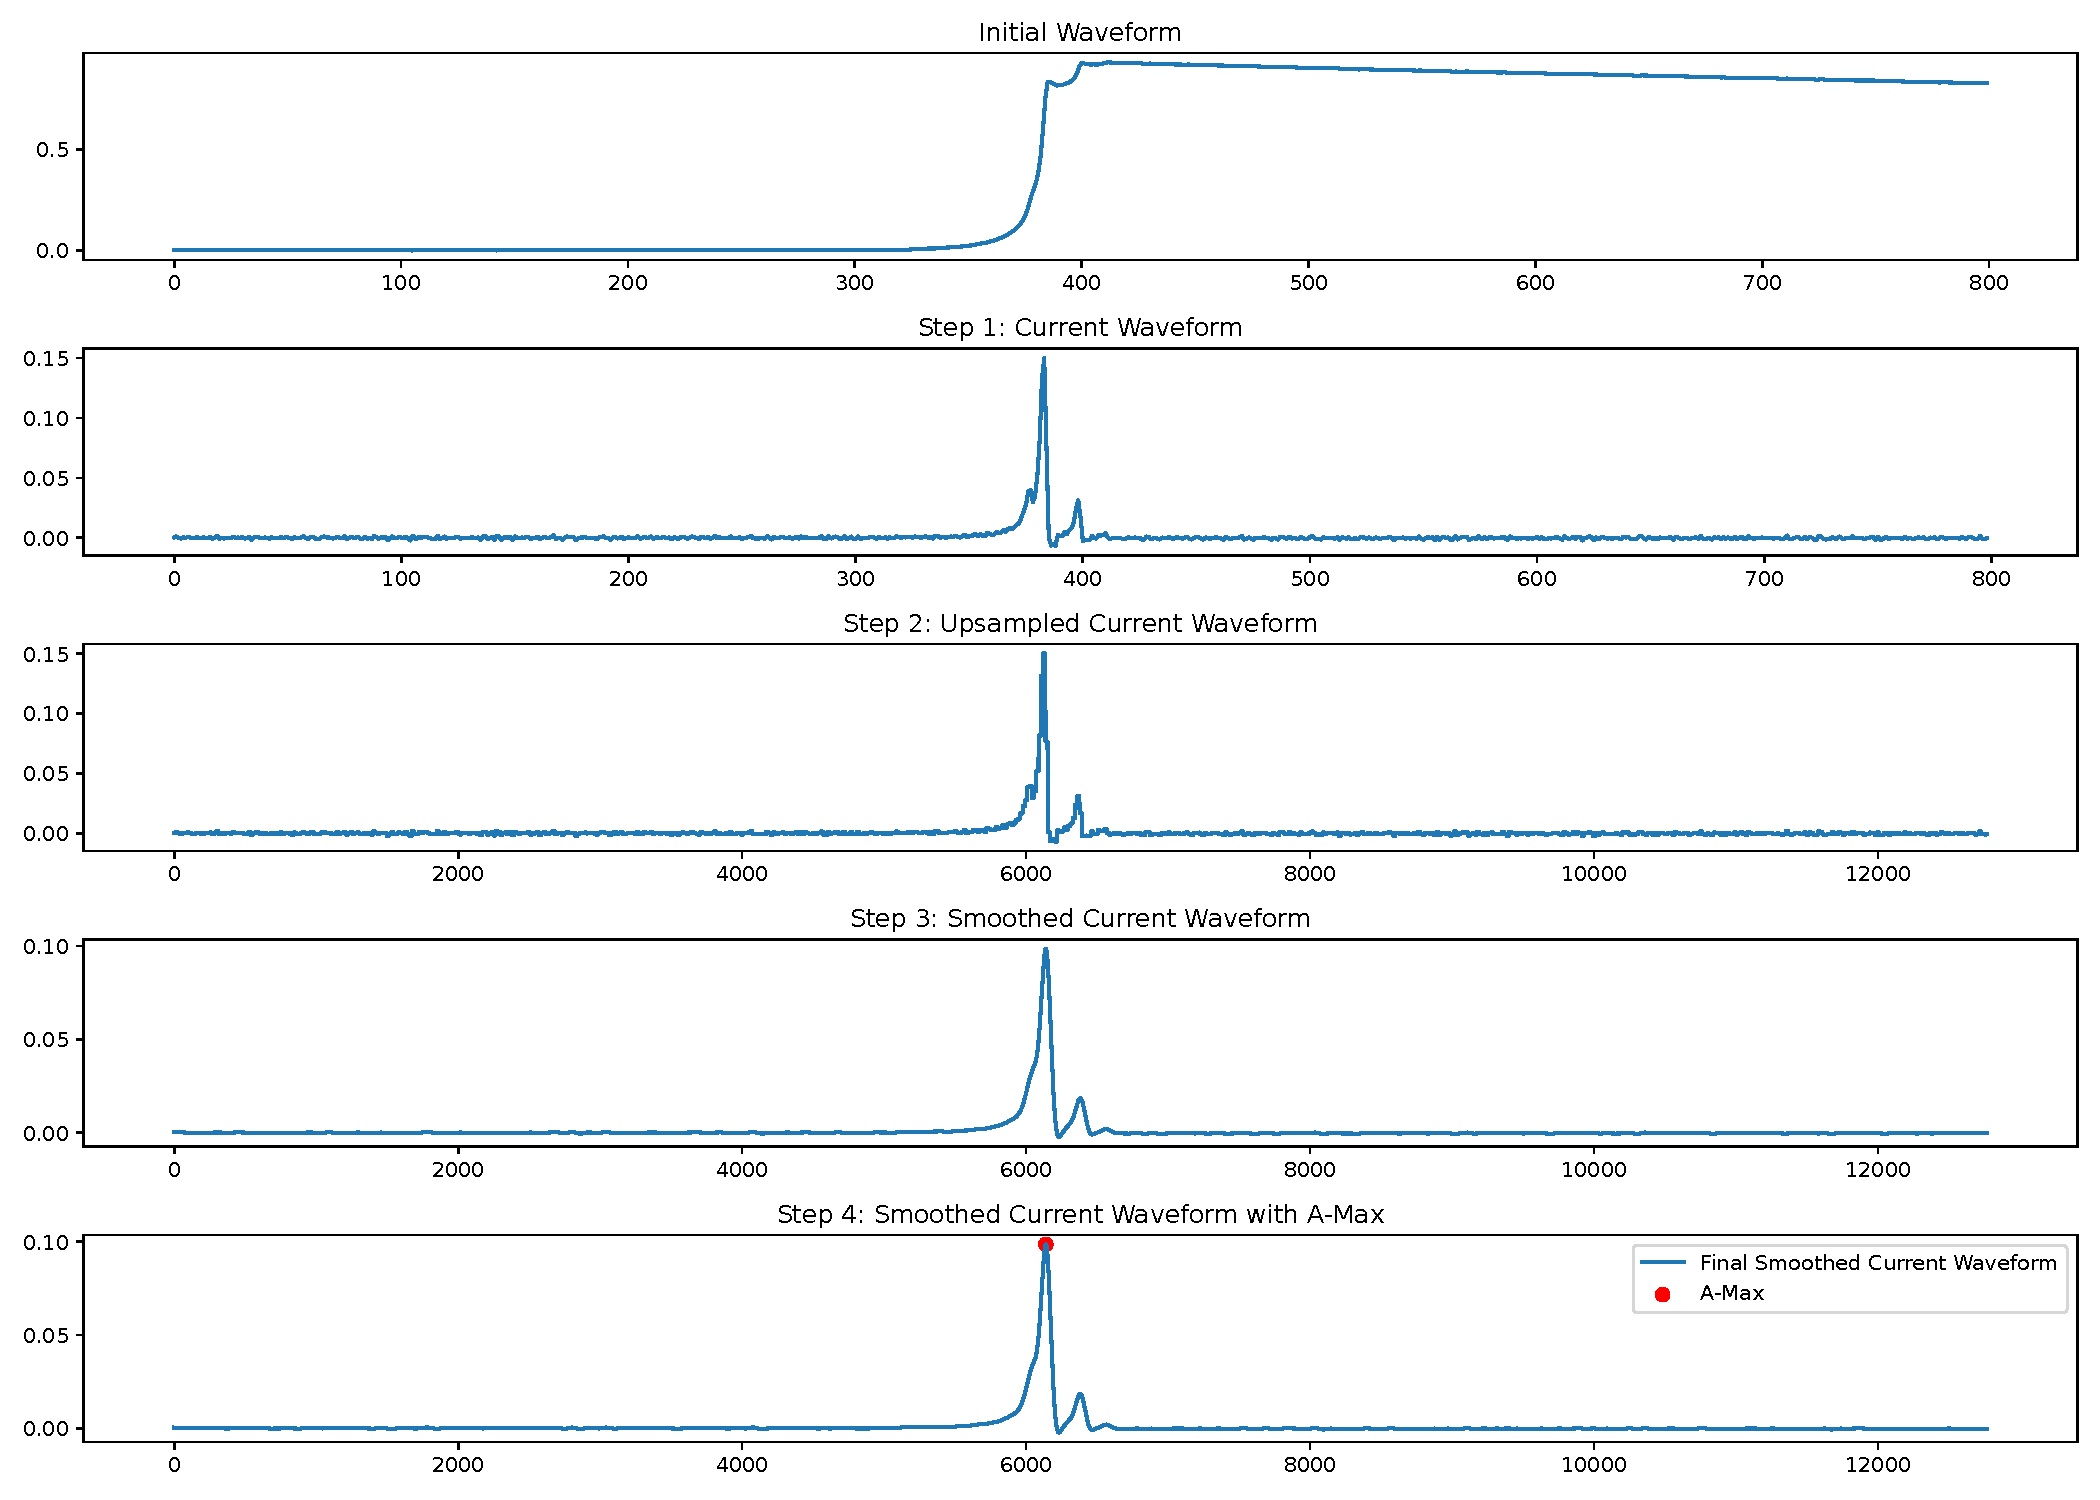
\includegraphics[width=0.99\linewidth, trim={0.4cm 0pc 0.3cm 0pc},clip]{ch8/figs/curr_amp_calc.pdf}
    \caption{Steps involved in calculating the maximum current amplitude of the waveform. First the discrete derivative of the waveform is calculated which is then up-sampled by a factor of 16 to extract finer detail. Then the current is smoothed to reduce the noise. The maximum value is $I_{max}$. The ratio of the $I_{max}$, to energy is used as a PSD parameter.}
    \label{fig_ch8_curr_amp_calc}
\end{figure}

Figures \ref{ch8_fig_current_amp_sep} and \ref{ch8_fig_current_amp_dep} illustrate the distribution of $I_{max}$ for both validation datasets. The SEP dataset distributions have two peaks, the higher of which corresponds to single-site events. The peak at a lower value of I$_max$ corresponds to multi-site events where one of the sites has an energy of 511 keV. DEP has only one peak for single-site events. ATN learns to correctly slow the current amplitude of the simulated waveforms to align with the data. The SEP $I_{max}$ increases to the IoU of $63.71\%$ from $27.53\%$. The DEP IoU increases to $15.5\%$ from $4.2\%$. 
  
\begin{figure}%[htb!]
\centering
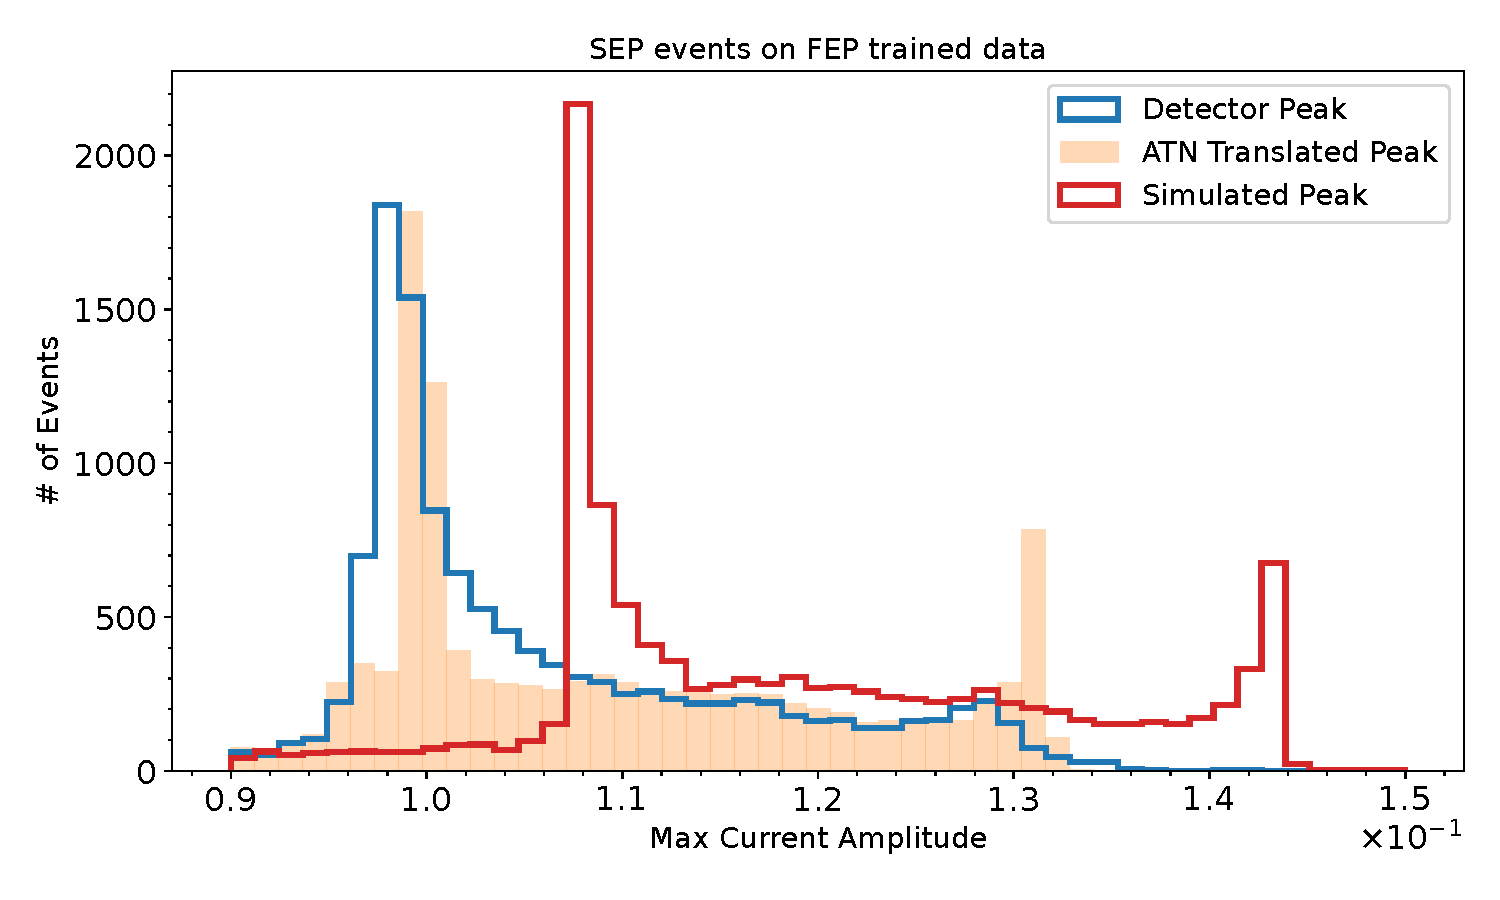
\includegraphics[width=0.9\linewidth,trim={0pc 0pc 0pc 0pc},clip]{ch8/figs/SEP_amp.pdf}
\caption{ Distribution of maximum current amplitude ($I_{max}$) on SEP validation datasets.}
\label{ch8_fig_current_amp_sep}
\end{figure}

\begin{figure}%[htb!]
\centering
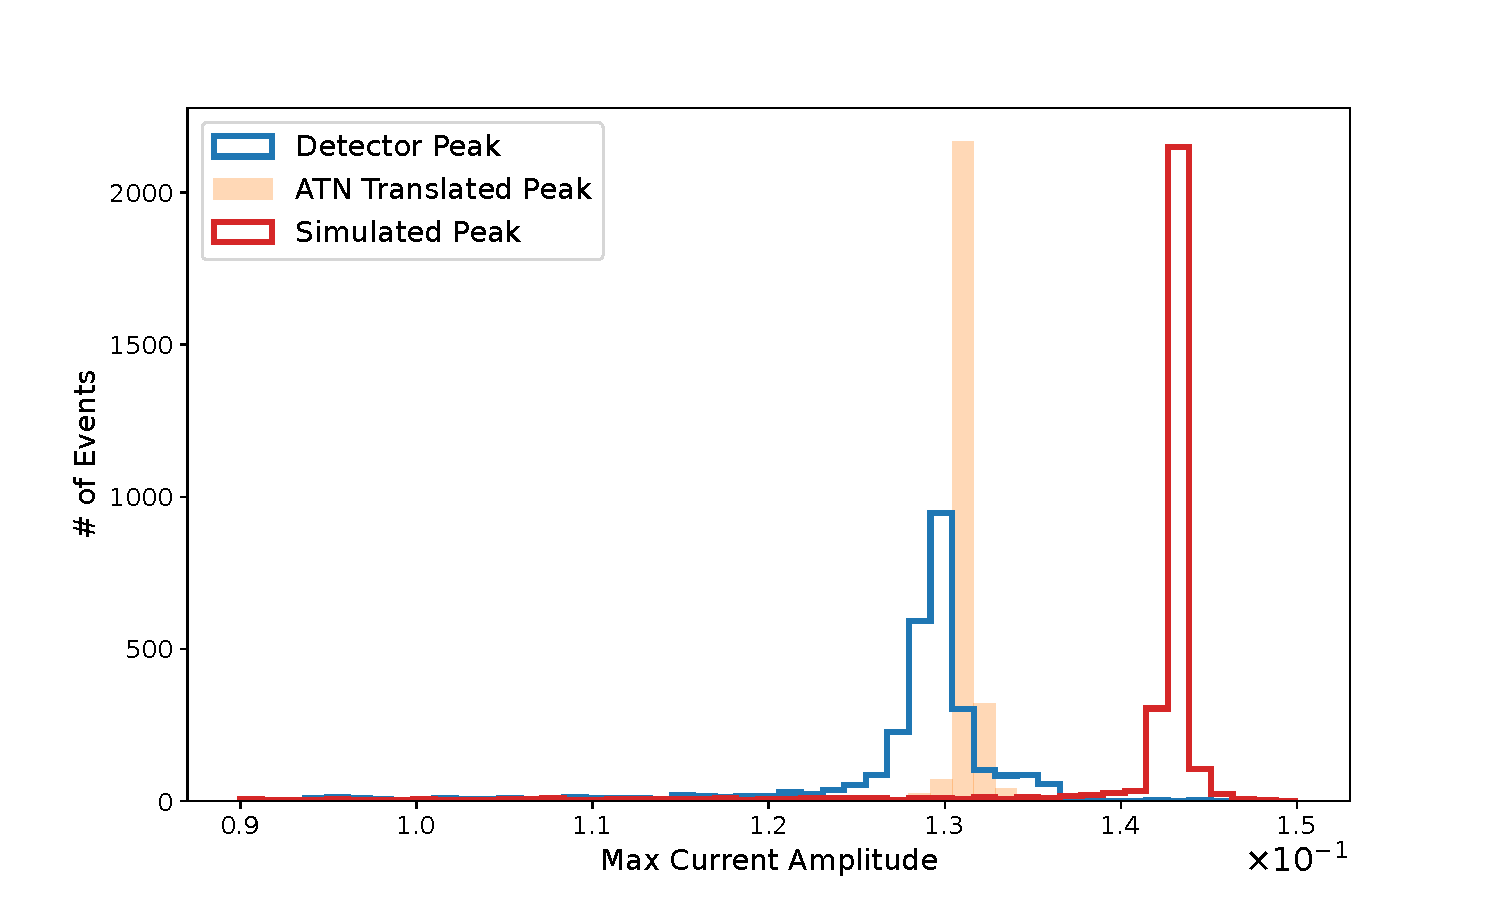
\includegraphics[width=0.9\linewidth,trim={0pc 0pc 0pc 0pc},clip]{ch8/figs/DEP_amp.pdf}
\caption{ Distribution of maximum current amplitude ($I_{max}$) on DEP validation datasets.}
\label{ch8_fig_current_amp_dep}
\end{figure}

Fig.\ref{ch8_fig_current_amp_sep} plots the $I_{max}$ of the ATN against $I_{max}$ of the simulated pulses. This shows that the ATN performs the translation while maintaining the relative order of the events. The waveforms are translated in a consistent way: waveforms that had the larger $I_{max}$ in the simulations have larger $I_{max}$ after translation. In other words, it is shifting the histogram instead of recreating it and reorganizing the events.

\begin{figure}%[htb!]
\centering
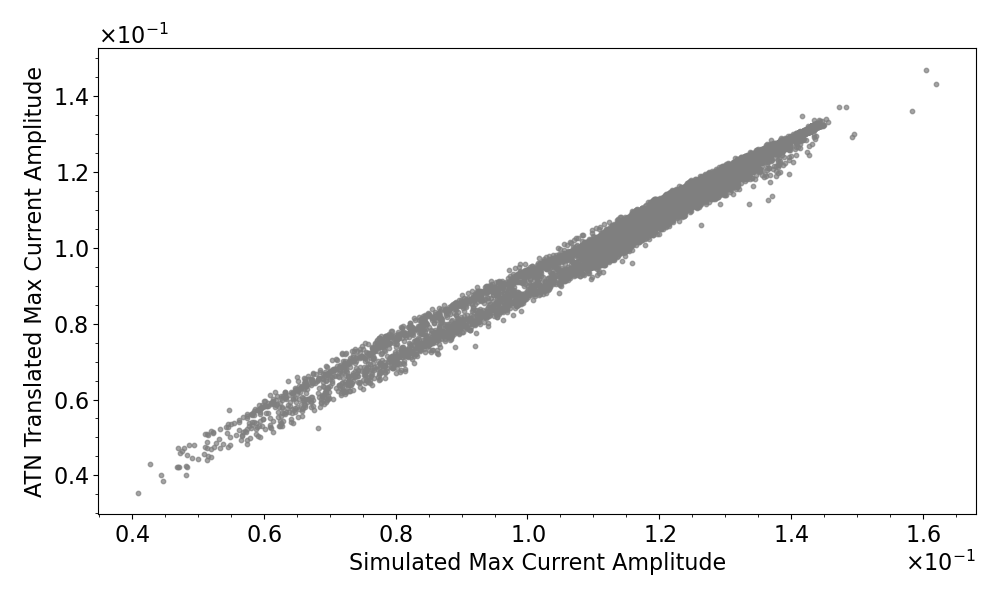
\includegraphics[width=0.9\linewidth,trim={0pc 0pc 0pc 0pc},clip]{ch8/figs/SEP_scatter_current_amplitude.png}
\caption{Scatter plot between $I_{max}$ of simulated waveforms and ATN translated waveforms. ATN shifts the amplitude distribution to align with data while maintaining the relative ordering of individual events.}
\label{fig:current_amp}
\end{figure}

{\cpunet} provides significant improvement in agreement between translated and data waveforms for drift time and current amplitude distributions. These agreements could likely be increased by using improved input simulations. The {\siggen} simulation includes heuristic models for diffusion and self-repulsion, but it treats each energy deposition as a single point charge, which can lead to overly similar shapes of single-site waveforms. Including actual charge cloud effects in the simulation can help incorporate effects due to cloud evolution during drift in the input simulations and improve the performance of the model.

\subsection{Tail Slope}
The strength of the RC decay can be measured by the mean tail slope parameter $c_{tail}$. Since the RC decay is an exponential decay, $c_{tail}$ was calculated by a linear fit of the logarithm of 300 samples of the waveform as shown in figure \ref{ch8_fig_tail_slope_calc}. The simulation waveforms do not have an RC decay and thus have a mean tail slope of zero. The data waveform was found to have a mean $c_{tail}$ of $-1.8605\times10^{-4}$ ADC/ns which is equal to a decay constant $\tau = 1/|c_{\mathrm{tail}}|$
 of $54.60 \mu s$, while the ATN translated waveform had a mean $c_{tail}$ of $-2.9769\times10^{-4}$ ADC/ns, which is equal to a $\tau$ of $53.75 \mu s$. This is a difference of $1.58\%$ from the actual value. Figure \ref{ch8_fig_tail_slope_comp} shows this relative magnitude of $c_{tail}$ for simulations, data, and ATN translated waveforms. Relative to the simulations, the distribution of ATN translated waveforms lies close to the data waveforms.

\begin{figure}%[!htb]
    \centering
    %trim={0pc 0pc 0pc 3pc},clip
    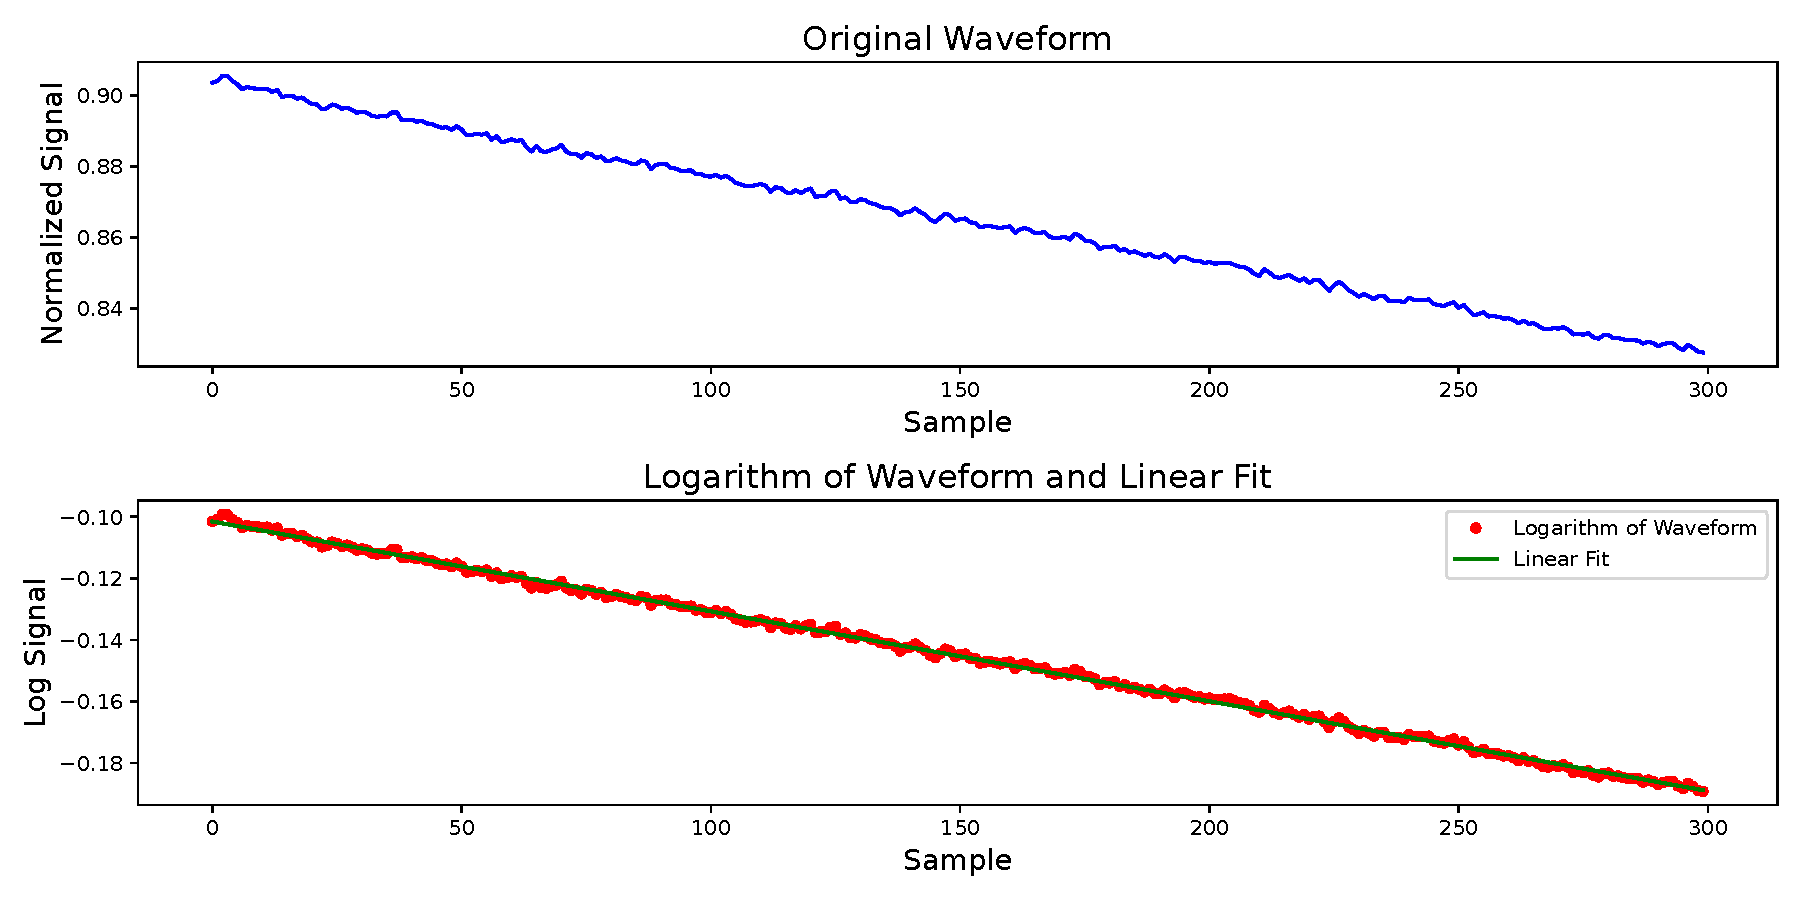
\includegraphics[width=0.99\linewidth, trim={0.4cm 0pc 0.3cm 0cm},clip]{ch8/figs/tail_slope_calc.pdf}
    \caption{Calculating the tail slope ($c_{tail}$) of the waveform. We take the logarithm of last 300 samples of the waveform and linear fit it to find the slope.}
    \label{ch8_fig_tail_slope_calc}
\end{figure}

\begin{figure}%[!htb]
\centering
%[trim={left bottom right top},clip]
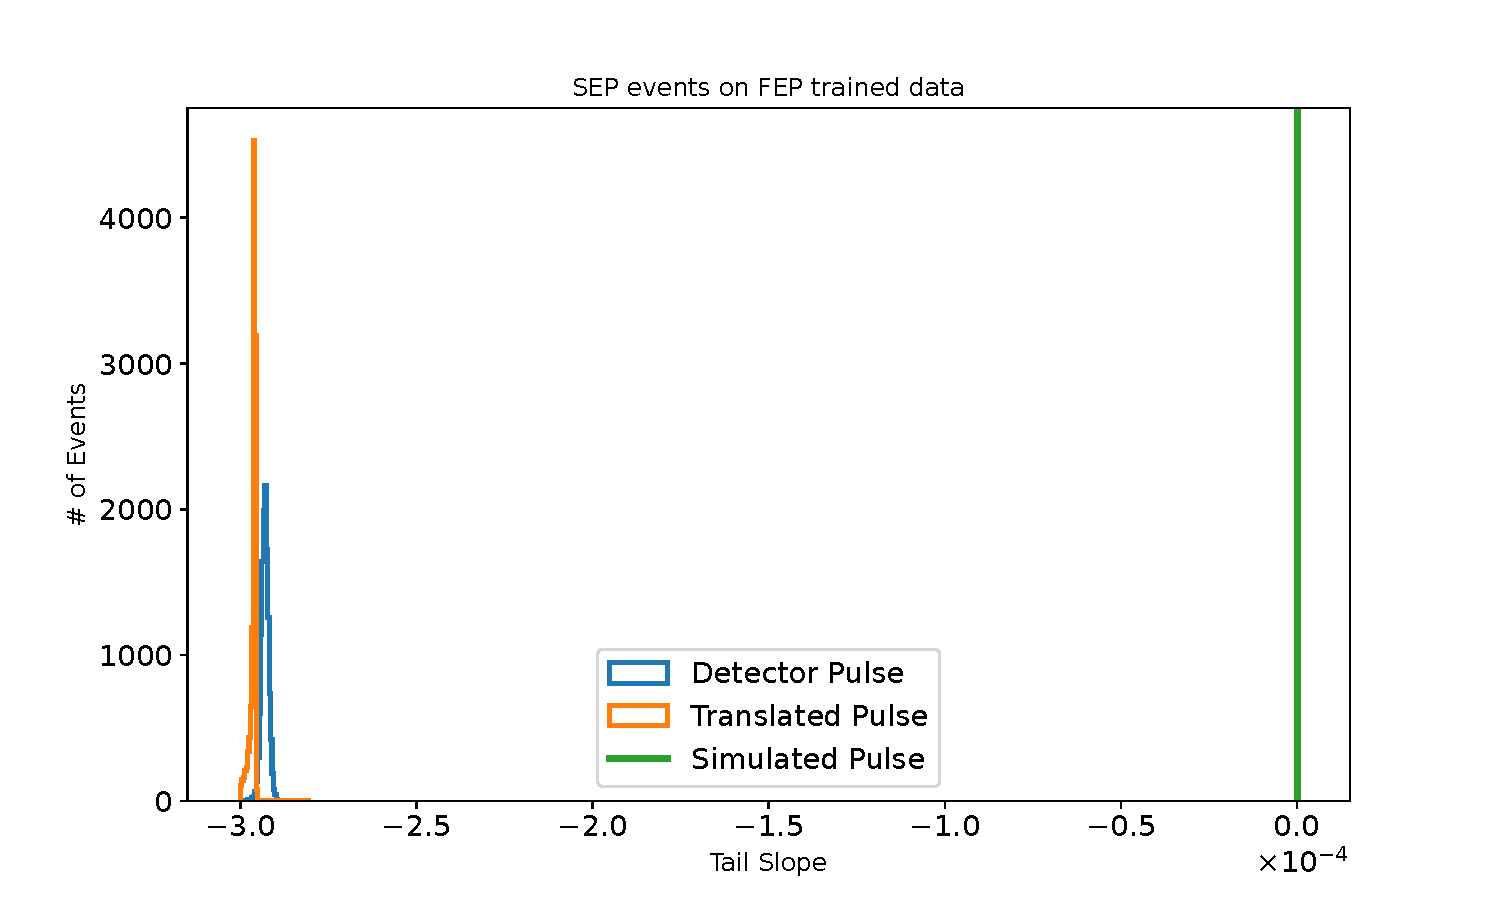
\includegraphics[width=0.9\linewidth,trim={2pc 0pc 2pc 0pc},clip]{ch8/figs/SEP_ts_with_sim.pdf}
\caption{Distribution of $c_{tail}$ for simulations, data, and ATN translated waveforms.}
\label{ch8_fig_tail_slope_comp}
\end{figure}

Figure \ref{ch8_fig_tail_slope_sim} shows the comparison of the $c_{tail}$ distribution between the data and the ATN translated waveforms. The distributions do not match perfectly, suggesting that the model is not learning this parameter distribution well. This could be a numerical precision issue since the tail slope magnitude is quite small. It could also be that at some step in training the generator determined that the RC decay tail it was adding to the simulated waveforms was enough to fool the discriminator and thus does not improve further to match the distribution of the data. In the next chapter, we suggest some ways to improve the model.

\begin{figure}%[!htb]
\centering
%[trim={left bottom right top},clip]
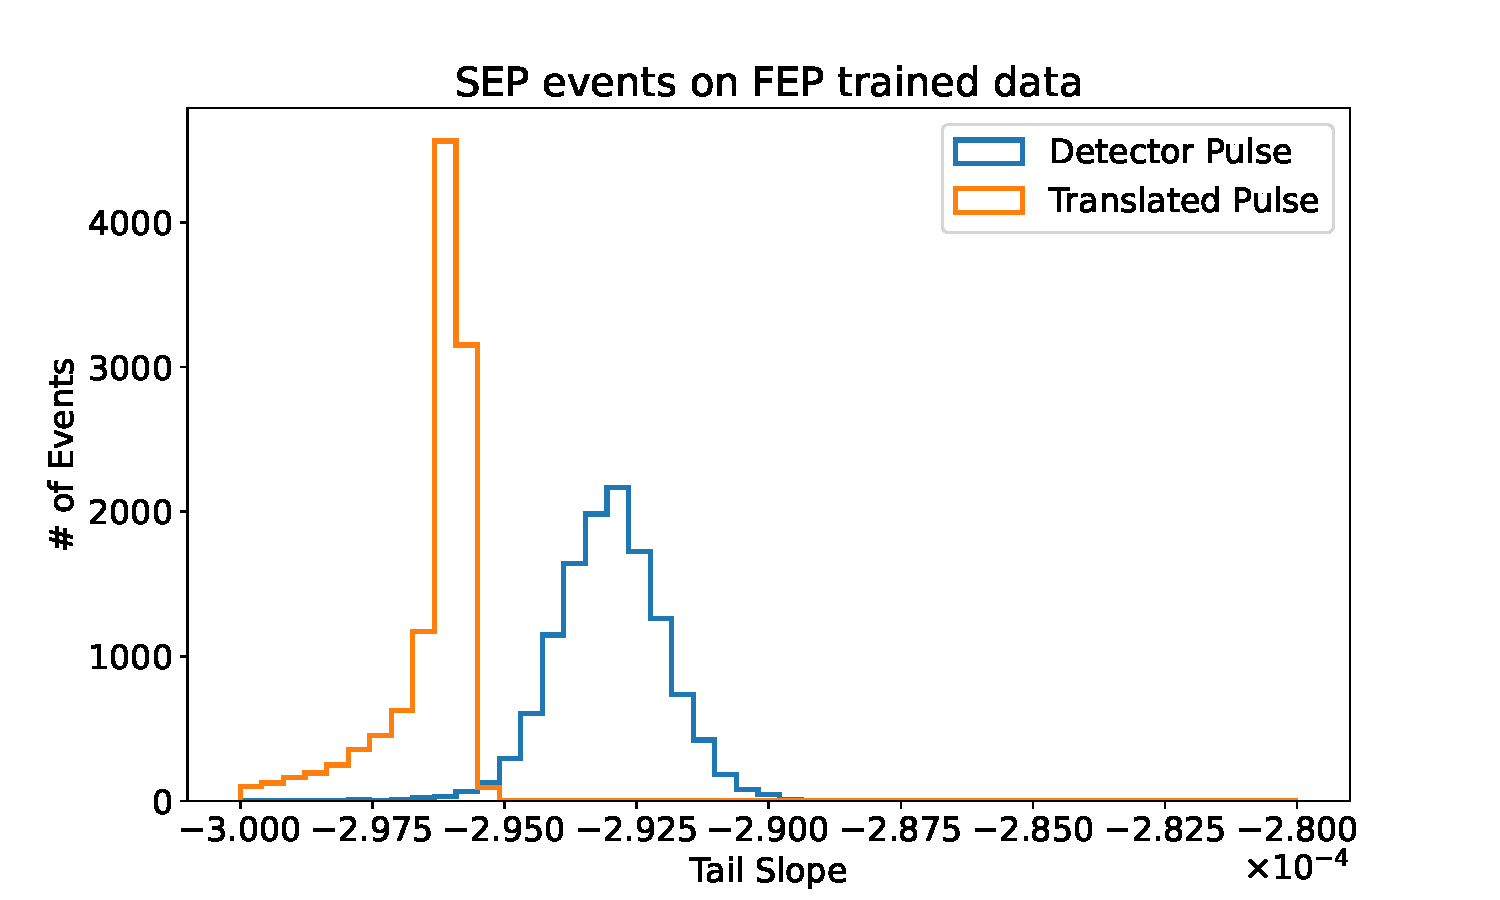
\includegraphics[width=0.9\linewidth,trim={2pc 0pc 2pc 0pc},clip]{ch8/figs/SEP_ts.pdf}
\caption{Distribution of tail slope ($c_{tail}$) between data and ATN translated waveforms.}
\label{ch8_fig_tail_slope_sim}
\end{figure}

Although our main focus in this work is on translating simulations to resemble measured data, {\cpunet}’s bidirectional nature also makes it a powerful tool for denoising real detector waveforms. By transforming noisy detector signals into cleaner, simulation-like waveforms, {\cpunet} can help isolate and identify subtle features in the event topology. This capability could ultimately improve spatial reconstruction and improve our understanding of particle interactions within the detector.

Electronics response modeling is necessary for accurate pulse shape simulations and is challenging to determine from first principles. {\cpunet} is a deep learning framework that is showing good performance in accurately translating simulated waveforms to match the data with the electronics response. The translations preserve the necessary physics and have shown success in reproducing waveform parameter distributions.
